\section{Logic, Shift and Rotate Instructions}

\section*{Logical Instructions}
The following instruction only affect N and Z flags

\begin{itemize}
  \item ANDS
  \item BICS
  \item EORS
  \item MVNS Bitwise NOT
  \item ORRS
\end{itemize}

Bitwise OR

Rdn \# Rm\\
Rdn \& Rm\\
Rdn \& ! Rm $\quad a \& \sim b$\\
Rdn \$ Rm $\quad a{ }^{\wedge} b$\\
Rm a\\
a | b

Shift Instructions

\begin{itemize}
  \item LSLS Logical Shift Left $\quad 2^{n} \cdot R n \quad 0 \rightarrow L S B$
  \item LSRS Logical Shift Right $\quad 2^{-n} \cdot R n \quad 0 \rightarrow M S B$
  \item ASRS Arithmetic Shift Right $\quad R^{-n} \pm \pm M S B \rightarrow M S B$
  \item RORS Rotate Right $\quad L S B \rightarrow M S B$\\
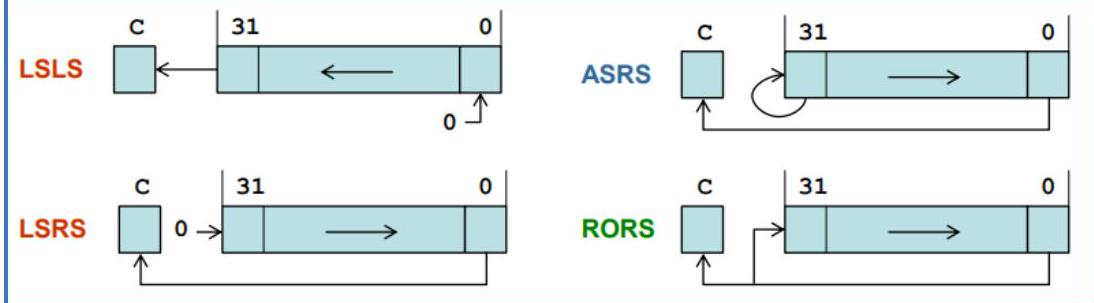
\includegraphics[max width=\textwidth, center]{2024_12_29_79e6b22f503fb7b4f718g-06}
\end{itemize}

\section*{Sign-Extension}
Add additional bits

\begin{itemize}
  \item Unsigned zero extension fill left bits with zero
  \item Signed sign extension copy sign bit to the left
\end{itemize}

\begin{center}
\begin{tabular}{|c|c|c|c|c|}
\hline
\multicolumn{2}{|l|}{Unsigned $\rightarrow \boldsymbol{\sim}$ Zero Extension} &  & \multirow[b]{2}{*}{$\rightarrow$} & \multirow[b]{2}{*}{00000011} \\
\hline
$1011 \rightarrow$ & 00001011 & 0011 &  &  \\
\hline
\multicolumn{5}{|l|}{Signed $\boldsymbol{\rightarrow}$ Sign Extension} \\
\hline
$1011 \rightarrow$ & 11111011 & 0011 & $\rightarrow$ & 00000011 \\
\hline
\end{tabular}
\end{center}

\section*{Truncation}
Cast cuts out the left most digits

\begin{itemize}
  \item Signed possible change of sign
  \item Unsigned results in module operation
\end{itemize}

\section*{Integer ranges based on word sizes}
\begin{center}
\begin{tabular}{|c|c|c|c|c|c|c|c|}
\hline
\multirow[t]{6}{*}{8-bit} & \( \begin{gathered} \text { hex } \\ 0 \times 00 \end{gathered} \) & unsigned & signed & 16-bit & hex 0×0000 & unsigned & signed \\
\hline
 &  &  &  &  &  &  &  \\
\hline
 & 0x75 & 127 & 127 &  & 0x7FFF & F 32'767 & $32 \cdot 767$ \\
\hline
 & 0x80 & 128 & -128 &  & 0x8000 & $032 \cdot 768$ & -32'768 \\
\hline
 &  & . . . & -. &  & . . & . . &  \\
\hline
 & 0xFF & 255 & -1 &  & 0xFFFF & F 65'535 & -1 \\
\hline
\multicolumn{2}{|r|}{\multirow[t]{7}{*}{32-bit}} & \multicolumn{2}{|l|}{hex} & \multicolumn{2}{|l|}{unsigned} & signed &  \\
\hline
 &  & \multicolumn{2}{|l|}{0x0000 0000} & \multicolumn{2}{|l|}{o} & 0 &  \\
\hline
 &  & \multicolumn{2}{|l|}{\multirow[t]{2}{*}{0x7FFF'FFFF}} & \multicolumn{2}{|l|}{\multirow[t]{2}{*}{2'147'483'647}} & ... &  \\
\hline
 &  &  &  &  &  & 2'147'483' &  \\
\hline
 &  & \multicolumn{2}{|l|}{0x8000'0000} & \multicolumn{2}{|l|}{2'147'483'648 -} & -2'147'483' &  \\
\hline
 &  & \multicolumn{2}{|l|}{\multirow[t]{2}{*}{0xFFFF'FFFF}} & \multicolumn{2}{|l|}{\multirow[t]{2}{*}{4'294'967'295}} & -. &  \\
\hline
 &  &  &  &  &  & -1 &  \\
\hline
\end{tabular}
\end{center}